\section{Chat}
Ogni peer della chat è un client/server multicast che si lega ad un \textit{multicast group} di riferimento per i gruppi di utenti che stanno editando sezioni appartenenti ad uno stesso documento: se non esistono su di esso, la relativa chat non dovrebbe concettualmente esistere.

\paragraph{Assegnazione Dinamica dei Gruppi Multicast}
Per implementare questo comportamento, ho scelto di generare e gestire gli indirizzi delle chat in maniera dinamica, attraverso un algoritmo di generazione molto semplice illustrato in figura \ref{fig:multicast_address_generation} . A gestire l'allocazione degli indirizzi è l'oggetto \textbf{CDAManager}\footnote{CDAManager := Chat Dynamic Address Manager.}. Questo si serve della rappresentazione intera decimale degli indirizzi IPv4 per maneggiarli in maniera più semplice e gestirne meglio l'incremento.

\begin{figure}[h]
	\caption{Activity Diagram - Generazione dinamica indirizzo di multicast}
	\label{fig:multicast_address_generation}
	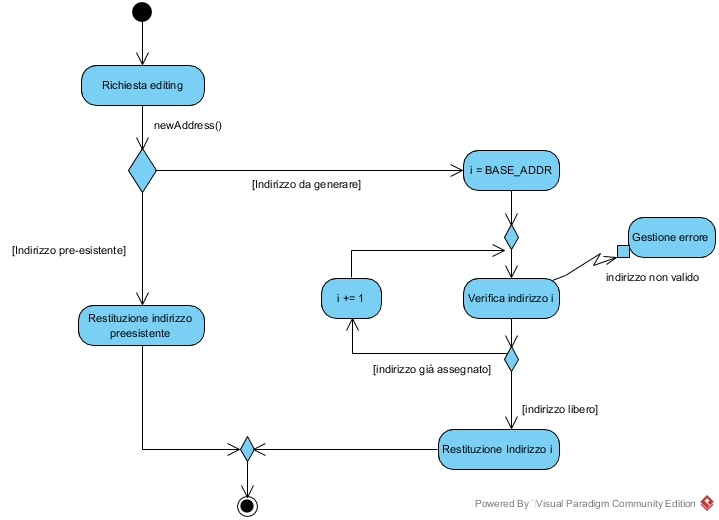
\includegraphics[scale=0.5]{assets/multicast_address_generation_algorithm.jpg}
\end{figure}

Quando tutti gli editor terminano la modifica della sezione, l'indirizzo diventa nuovamente disponibile e riutilizzabile da un altro gruppo multicast.

\paragraph{Comunicazione tra i Client}
Il server TURING non gioca alcun ruolo nella comunicazione tramite il servizio di chat se non quello di fornire, come descritto in precedenza, l'indirizzo di multicast relativo al canale del documento che si sta editando. Questa struttura ha permesso di snellire il processo di funzionamento del servizio, evitando di interporre inutilmente il server in funzione di \textit{proxy} delle richieste tra i fruitori.

I messaggi vengono ricevuti dall'oggetto \textbf{MessageReceiver} e inviati tramite il \textbf{MessageSender}, incapsulando le informazioni all'interno di \textbf{ChatMessage}. I messaggi ricevuti vengono immagazzinati all'interno di una struttura interna al receiver, che li mantiene fino a quando non ne viene richiesto il contenuto in maniera \underline{asincrona} attraverso il comando \textit{receive}. A quel punto, i messaggi vengono riordinati temporalmente\footnote{Viene sfruttato il campo \textbf{time} e l'interfaccia \textbf{Comparable} della classe \textbf{ChatMessage} per ripristinare l'ordine originale di invio dei messaggi in caso di ritardo di ricezione.} e stampati a schermo. Una volta stampati, i messaggi vengono persi e non mantenuti in memoria da alcun nodo.